\documentclass{beamer}

\mode<presentation> {

%\usetheme{default}
%\usetheme{AnnArbor}
%\usetheme{Antibes}
%\usetheme{Bergen}
%\usetheme{Berkeley}
%\usetheme{Berlin}
%\usetheme{Boadilla}
%\usetheme{CambridgeUS}
%\usetheme{Copenhagen}
%\usetheme{Darmstadt}
%\usetheme{Dresden}
%\usetheme{Frankfurt}
%\usetheme{Goettingen}
%\usetheme{Hannover}
%\usetheme{Ilmenau}
%\usetheme{JuanLesPins}
%\usetheme{Luebeck}
\usetheme{Madrid}
%\usetheme{Malmoe}
%\usetheme{Marburg}
%\usetheme{Montpellier}
%\usetheme{PaloAlto}
%\usetheme{Pittsburgh}
%\usetheme{Rochester}
%\usetheme{Singapore}
%\usetheme{Szeged}
%\usetheme{Warsaw}


%\usecolortheme{albatross}
%\usecolortheme{beaver}
%\usecolortheme{beetle}
%\usecolortheme{crane}
%\usecolortheme{dolphin}
%\usecolortheme{dove}
%\usecolortheme{fly}
%\usecolortheme{lily}
%\usecolortheme{orchid}
%\usecolortheme{rose}
%\usecolortheme{seagull}
%\usecolortheme{seahorse}
%\usecolortheme{whale}
%\usecolortheme{wolverine}

%\setbeamertemplate{footline} % To remove the footer line in all slides uncomment this line
%\setbeamertemplate{footline}[page number] % To replace the footer line in all slides with a simple slide count uncomment this line

%\setbeamertemplate{navigation symbols}{} % To remove the navigation symbols from the bottom of all slides uncomment this line
}

\usepackage{graphicx} % Allows including images
\usepackage{booktabs} % Allows the use of \toprule, \midrule and \bottomrule in tables
\usepackage{amsfonts}
\usepackage{mathrsfs, bbold}
\usepackage{amsmath,amssymb,graphicx}
\usepackage{mathtools} % gather

\newcommand{\sbf}{\boldsymbol}

%----------------------------------------------------------------------------------------
%	TITLE PAGE
%----------------------------------------------------------------------------------------

\title["3"]{3: Introduction to multiparameter models}

% \author{Taylor} 
% \institute[UVA] 
% {
% University of Virginia \\
% \medskip
% \textit{} 
% }
\date{09/03/19} 

\begin{document}
%----------------------------------------------------------------------------------------

\begin{frame}
\titlepage 
\end{frame}

%----------------------------------------------------------------------------------------
\begin{frame}
\frametitle{Introduction}

We discuss a few examples of models with more than one parameter.


\end{frame}


%----------------------------------------------------------------------------------------
\begin{frame}
\frametitle{A noninformative prior with a normal likelihood}

Consider a normal likelihood
\begin{align*}
p(y \mid \mu, \sigma^2) &\propto (\sigma^2)^{-n/2}\exp\left[ - \frac{1}{2\sigma^2} \sum_i(y_i- \mu)^2 \right] \\
&= (\sigma^2)^{-n/2}\exp\left[ - \frac{1}{2\sigma^2} \sum_i([y_i- \bar{y}] + [\bar{y} - \mu])^2 \right] \\
&= (\sigma^2)^{-n/2}\exp\left[ - \frac{1}{2\sigma^2} \left\{ \sum_i(y_i- \bar{y})^2 + n(\bar{y} - \mu)^2 + 0 \right\} \right] \\
&= (\sigma^2)^{-n/2} \exp\left[ - \frac{1}{2\sigma^2}\left\{(n-1)  s^2 + n(\bar{y} - \mu)^2 \right\} \right]
\end{align*}

and the noninformative, improper prior $p(\mu, \sigma^2) \propto \sigma^{-2}$. Clearly 
\[
p(\mu, \sigma^2 \mid y) \propto (\sigma^2)^{-(n+2)/2}\exp\left[ - \frac{1}{2\sigma^2}\left\{(n-1)  s^2 + n(\bar{y} - \mu)^2 \right\} \right]
\]

\end{frame}


%----------------------------------------------------------------------------------------
\begin{frame}
\frametitle{A noninformative prior with a normal likelihood}

Suppose that $\mu$ is a nuisance parameter, and we're only interested in $\sigma^2$. Then, we want he marginal posterior:
\begin{align*}
p(\sigma^2 \mid y) &\propto \int (\sigma^2)^{-(n+2)/2} \exp\left[ - \frac{1}{2\sigma^2}\left\{(n-1)  s^2 + n(\bar{y} - \mu)^2 \right\} \right] \text{d}\mu \\
&= (\sigma^2)^{-(n+2)/2}  \exp\left[ - \frac{(n-1)}{2\sigma^2}s^2  \right] \int \exp\left[ - \frac{1}{2\sigma^2} n(\mu - \bar{y} )^2 \right] \text{d}\mu \\
&\propto (\sigma^2)^{-(n+2)/2}  \exp\left[ - \frac{(n-1)}{2\sigma^2}s^2  \right] (\sigma^2)^{1/2} \\
&= (\sigma^2)^{-[(n-1)/2 + 1]}  \exp\left[ - \frac{(n-1)s^2}{2\sigma^2}  \right] 
\end{align*}

$\sigma^2 \mid y \sim \text{Inv-Gamma}\left(\frac{n-1}{2}, \frac{(n-1)s^2}{2}\right)$
\end{frame}



%----------------------------------------------------------------------------------------
\begin{frame}
\frametitle{A noninformative prior with a normal likelihood}

Recall the joint posterior:
\[
p(\mu, \sigma^2 \mid y) \propto (\sigma^2)^{-(n+2)/2}\exp\left[ - \frac{1}{2\sigma^2}\left\{(n-1)  s^2 + n(\bar{y} - \mu)^2 \right\} \right]
\]

Clearly:
\[
p(\mu \mid \sigma^2, y) \propto \exp\left[ - \frac{n}{2\sigma^2} (\bar{y} - \mu)^2  \right]
\]
\pause

We also have $p(\sigma^2 \mid y)$ from the last slide. This means that we can figure out the normalizing constants for the joint posterior if we multiply these two known densities together:
\[
p(\mu, \sigma^2 \mid y) = p(\mu \mid \sigma^2,y) p(\sigma^2 \mid y).
\]
Sometimes this is called a {\bf normal-inverse-gamma} distribution.

\end{frame}


%----------------------------------------------------------------------------------------
\begin{frame}
\frametitle{A noninformative prior with a normal likelihood}

Suppose instead that $\sigma^2$ is a nuisance parameter, and we're only interested in $\mu$. Then, we want the marginal posterior.
\newline

Let $z = \frac{1}{2\sigma^2}\left\{(n-1)  s^2 + n(\bar{y} - \mu)^2 \right\} = \frac{A}{2\sigma^2}$. Then
\begin{align*}
p(\mu \mid y) &\propto \int_0^{\infty} (\sigma^2)^{-(n+2)/2} \exp\left[ - \frac{1}{2\sigma^2}\left\{(n-1)  s^2 + n(\bar{y} - \mu)^2 \right\} \right] \text{d} \sigma^2 \\
&= \int_{\infty}^0 (A/2)^{-(n+2)/2}z^{(n+2)/2} \exp\left[ - z \right] (-A/2)z^{-2}\text{d} z \\
&= (A/2)^{-n/2} \underbrace{\int^{\infty}_0 z^{n/2-1} \exp\left[ - z \right] \text{d} z}_{\Gamma(n/2)} \\
\end{align*}
% so $\mu \mid y \sim t_{n-1}(\bar{y}, s^2/n)$ 


\end{frame}

%----------------------------------------------------------------------------------------
\begin{frame}
\frametitle{A noninformative prior with a normal likelihood}

So
\begin{align*}
p(\mu | y) &\propto (A/2)^{-n/2} \\
&\propto A^{-n/2} \\
&\propto A^{-n/2}[(n-1)  s^2]^{n/2} \\
&\propto \left(1 + \frac{(\bar{y} - \mu)^2}{(n-1)  s^2/n} \right)^{-n/2} 
\end{align*}
$\mu \mid y \sim t_{n-1}(\bar{y}, s^2/n)$, that is, $\frac{\mu -
  \bar{y}}{s/\sqrt{n}} \mid y \sim t_{n-1}$   
% &\propto \int \left( \frac{1}{2z}A \right)^{-(n+2)/2 + 2} \exp\left[ - z \right] A^{-1} \text{d} z \\
% &\propto A^{-n/2} \int z ^{(n-2)/2 } \exp\left[ - z \right]  \text{d} z \\
% &\propto \left\{(n-1)  s^2 \right\}^{-n/2} \left\{1 + \frac{n(\bar{y} - \mu)^2}{ (n-1)  s^2} \right\}^{-n/2} 

\end{frame}


% %----------------------------------------------------------------------------------------
% \begin{frame}
% \frametitle{A noninformative prior with a normal likelihood}

% After we have figured out the joint posterior, we may be interested in predicting new observations with the {\bf posterior predictive distribution}:
% \[
% p(\tilde{y} \mid y) = \iint p(\tilde{y} \mid \mu, \sigma^2) p(\mu, \sigma^2 \mid y) \text{d} \mu \text{d} \sigma^2.
% \]
% \pause

% We can simulate $\tilde{y}_i$ as follows:
% \begin{enumerate}
% \item draw $\sigma^2_i \mid y \sim p(\sigma^2 \mid y)$
% \item draw $\mu_i \mid \sigma^2_i, y \sim p(\mu \mid \sigma^2_i, y)$
% \item draw $\tilde{y}_i \mid \mu_i, \sigma^2_i \sim p(\tilde{y} \mid \mu_i, \sigma^2_i)$
% \end{enumerate}


% \end{frame}


%----------------------------------------------------------------------------------------
\begin{frame}
\frametitle{A noninformative prior with a normal likelihood}

After we have figured out the joint posterior, we may be interested in predicting new observations with the {\bf posterior predictive distribution}:
\[
p(\tilde{y} \mid y) = \iint p(\tilde{y} \mid \mu, \sigma^2) p(\mu, \sigma^2 \mid y) \text{d} \mu \text{d} \sigma^2.
\]

It's a homework question to show that 
\[
\tilde{y} \mid y \sim t_{n-1}\left(\bar{y}, s^2\left(1 + \frac{1}{n} \right) \right)
\]

\end{frame}

%----------------------------------------------------------------------------------------
\begin{frame}
\frametitle{A noninformative prior with a normal likelihood}

Let's get some practice simulating predictions, which will come in handy when we are dealing with more complicated scenarios where a closed-form posterior predictive distribution isn't available. We can simulate each $\tilde{y}_i$  as follows:

\begin{block}{Sampling Strategy}
For $i=1,2,\ldots$
\begin{enumerate}
\item draw $\sigma^2_i \mid y \sim p(\sigma^2 \mid y)$
\item draw $\mu_i \mid \sigma^2_i, y \sim p(\mu \mid \sigma^2_i, y)$
\item draw $\tilde{y}_i \mid \mu_i, \sigma^2_i \sim p(\tilde{y} \mid \mu_i, \sigma^2_i)$
\end{enumerate}
\end{block}

Each triple $(\tilde{y}_i, \mu_i, \sigma^2_i) \sim p(\tilde{y}, \mu, \sigma^2 \mid y) = p(\tilde{y} \mid \mu, \sigma^2) p(\mu \mid \sigma^2 \mid y)p(\sigma^2 \mid y)$.
\newline

So $ \tilde{y}_i \sim p(\tilde{y} \mid y) = \iint p(\tilde{y} \mid \mu, \sigma^2) p(\mu, \sigma^2 \mid y) \text{d} \mu \text{d} \sigma^2$



\end{frame}

% %----------------------------------------------------------------------------------------
% \begin{frame}
% \frametitle{Tip 1: If the joint is easier to sample from}

% If you simulate $(\tilde{y}^i, \theta_1^i, \theta_2^i)_{i=1}^n \sim p(\tilde{y}, \theta_1, \theta_2 \mid y)$, then ignoring pieces of each sample is analogous to sampling from the marginal:

% \[
% n^{-1}\sum_{i=1}^n h(\tilde{y}^i) \to E_{\tilde{y}, \theta_1, \theta_2}[h(\tilde{y}^i)] = E_{\tilde{y}}[h(\tilde{y}^i)]
% \]
% \end{frame}


% %----------------------------------------------------------------------------------------
% \begin{frame}
% \frametitle{Tip 2: if the ``top" factor of a joint is tractable}

% If $p(\tilde{y}, \theta_1, \theta_2 \mid y) = p(\tilde{y} \mid \theta_1, \theta_2, y) p(\theta_1,  \theta_2 \mid y)$, then

% \begin{align*}
% n^{-1} \sum_{i=1}^n E[h(\tilde{y}, \theta_1^i, \theta_2^i)  \mid \theta_1^i, \theta_2^i, y] &\to E\left( E[h(\tilde{y}, \theta_1, \theta_2)  \mid \theta_1, \theta_2, y]\right) \\
% &= E[h(\tilde{y}, \theta_1, \theta_2) \mid y]
% \end{align*}

% If you can derive expectations of $p(\tilde{y} \mid \theta_1, \theta_2, y)$, and you can sample from the other piece, then this {\bf Rao-Blackwellization} or {\bf marginalization} strategy can be a useful variance reduction technique.

% \end{frame}
 

% %----------------------------------------------------------------------------------------
% \begin{frame}[fragile]
% \frametitle{A comparison in R}

% See \verb|3.r| for details:

% \begin{center}
% 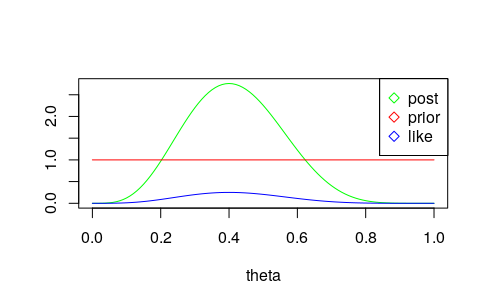
\includegraphics[width=100mm]{pics/Rplot}
% \end{center}


% \end{frame}
%----------------------------------------------------------------------------------------
\begin{frame}[fragile]
\frametitle{A conjugate prior with a normal likelihood}

Consider a normal likelihood again
\[
p(y \mid \mu, \sigma^2) = (\sigma^2)^{-n/2} \exp\left[ - \frac{1}{2\sigma^2}\left\{(n-1)  s^2 + n(\bar{y} - \mu)^2 \right\} \right]
\]

and an informative prior 
\begin{align*}
p(\mu, \sigma^2) &\propto \underbrace{\left(\frac{\sigma^2}{\kappa_0}\right)^{-1/2}\exp\left(-\frac{\kappa_0}{2 \sigma^2}(\mu - \mu_0)^2 \right)}_{p(\mu \mid \sigma^2)} \underbrace{(\sigma^2)^{-(\nu_0/2 + 1)} \exp\left(-\frac{\sigma^2_0 \nu_0}{2 \sigma^2} \right) }_{p(\sigma^2)} \\
&= (\sigma^2)^{-(\frac{\nu_0+1}{2} + 1)} \exp\left(-\frac{1}{2 \sigma^2}\left\{ \sigma^2_0 \nu_0 + \kappa_0(\mu - \mu_0)^2\right\} \right) 
\end{align*}
This is a {\bf normal-inverse-gamma} or $\mbox{{\bf
  normal-inverse-}}\chi^2(\mu_0, \sigma_0^2/\kappa_0; \nu_0, \sigma_0^2)$!

What are $p(\mu, \sigma^2 \mid y) ?, p(\mu \mid y) ?$

\end{frame}

%----------------------------------------------------------------------------------------
\begin{frame}[fragile]
\frametitle{Another multiparameter example of conjugacy: Dirichlet-multinomial}

Let $y = (y_1, y_2, \ldots, y_k)$ be a vector of counts. Let $\theta = (\theta_1, \theta_2, \ldots, \theta_k)$ be the probabilities of any trial resulting in each of the $k$ outcomes. We assume that there is a known total count (which means $\sum_i y_i = n$) and that the only possible outcomes are these $k$ outcomes $\sum_i \theta_i = 1$.
\newline

The likelihood is a {\bf multinomial} (aka a {\bf categorical}) distribution
$$
p(y \mid \theta) \propto \prod_{i=1}^k \theta_i^{y_i},
$$
and the prior is a Dirichlet distribution
$$
p(\theta) \propto \prod_{i=1}^k \theta_i^{\alpha_i - 1}.
$$
The chosen hyper-parameters have a very nice interpretation of counts!
\end{frame}

%----------------------------------------------------------------------------------------
\begin{frame}
  \frametitle{Dirichlet-multinomial }
Denote Dirichlet distribution as $\mbox{Dirichlet}(\alpha_1, \alpha_2, \ldots,
\alpha_k)$
$$
p(\theta) \propto \prod_{i=1}^k \theta_i^{\alpha_i - 1}.
$$
$$
p(\theta \mid y) \propto \prod_{i=1}^k \theta_i^{\alpha_i + y_i - 1}
$$  
$p(\theta \mid y) \sim \mbox{Dirichlet}(\alpha_1 + y_1, \ldots,
\alpha_k + y_k)$

\begin{itemize}
\item Dirichlet distribution has support on a simplex
  $\mathcal{S} = \{\sbf{\theta}=(\theta_1,\ldots,\theta_k): \sum_{i=1}^k \theta_i =
  1\}$
\item $k = 2$, $\mbox{Dirichlet}(\alpha_1,\alpha_2)$ becomes $\mbox{Beta}(\alpha_1, \alpha_2)$.
\item Like Beta distribution, when $\alpha_i = 1$
  it becomes a uniform distribution on $\mathcal{S}$; when $\alpha_i =
  0$ it is an improper prior and is equivalent to assigning a uniform
  prior on $\log(\theta_i)$ with the constraint that $\sbf{\theta} \in
  \mathcal{S}$.
\end{itemize}
\end{frame}


% %----------------------------------------------------------------------------------------
% \begin{frame}[fragile]
% \frametitle{A few notes on example 3.7}

% \begin{enumerate}
% \item It's a logistic regression model with two parameters: slope and intercept
% \item Groups: $i=1,2,3,4$
% \item For each group, sample size $n_i$ is known
% \item For each group, $y_i$ is a count (tumors, deaths, etc.)
% \item For each group, $x_i$ is a dose (continuous amount of treatment for each group)
% \end{enumerate}

% \end{frame}

% %----------------------------------------------------------------------------------------
% \begin{frame}[fragile]
% \frametitle{A few notes on example 3.7}

% For each group:
% \begin{gather*}
% y_i \mid \alpha, \beta \sim \text{Binomial}(n_i, \text{invlogit}(\alpha + \beta x_i))
% \end{gather*}

% We can write $\theta_i = \text{invlogit}(\alpha + \beta x_i)$ to make it cleaner, but note that this isn't introducing more parameters. The likelihood is
% $$
% p(y \mid \alpha, \beta) = \prod_{i=1}^4 \theta_i^{y_i}(1-\theta_i)^{n_i-y_i}
% $$


% \end{frame}

% %----------------------------------------------------------------------------------------
% \begin{frame}[fragile]
% \frametitle{A few notes on example 3.7}

% For each group:
% \begin{gather}
% y_i \mid \alpha, \beta \sim \text{Binomial}(n_i, \text{invlogit}(\alpha + \beta x_i))
% \end{gather}


% \begin{enumerate}
% \item The {\bf dose-response} is the relationship between $x_i$ and $\theta_i$ (which is assumed the same for each group $i$).
% \item {\bf LD-50} is the unknown quantity $-\alpha/\beta$. It only makes sense when $\beta > 0$, and it is the value of $x_i$ that yields $\theta_i = .5$ (plug it into eqn (1) above). Sometimes scientists are more interested in estimating this than they are in estimating individual parameters.
% \end{enumerate}

% \end{frame}


% %----------------------------------------------------------------------------------------
% \begin{frame}[fragile]
% \frametitle{A few notes on example 3.7}

% We assume an improper prior: $p(\alpha,\beta) \propto 1$. So
% \begin{align*}
% &\log p(\alpha,\beta \mid y) \\
% &= c + \log p(y \mid \alpha, \beta) + \log p(\alpha,\beta) \\
% &= c +  \log\prod_{i=1}^4 \theta_i^{y_i}(1-\theta_i)^{n_i-y_i} \\
% &= c +  \log\prod_{i=1}^4 \left(\frac{\theta_i}{(1-\theta_i)}\right)^{y_i}(1-\theta_i)^{n_i} \\
% &= c + \sum_{i=1}^4 y_i (\alpha + \beta x_i) - n_i\log[1 + \exp (\alpha + \beta x_i)] \\
% \end{align*}


% \begin{enumerate}
% \item One of the authors has provided \verb|R| code: \url{https://github.com/avehtari/BDA_R_demos/tree/master/demos_ch3}
% \end{enumerate}

% \end{frame}


\end{document} 


%%% Local Variables:
%%% mode: latex
%%% TeX-master: t
%%% End:
